\section{\our Overview}
\label{sec:hindsight-overview}

\our is a memory architecture for AI agents that unifies long-term factual recall with preference-conditioned reasoning. Each agent is backed by a memory bank that accumulates interactions encountered over time, and a reasoning layer that uses this memory to answer questions, form opinions, and update its beliefs in a consistent way. 
%Conceptually, \our ties together two components: TEMPR, which focuses on memory storage and retrieval, and CARA, which focuses on preference-aware reflection.

\subsection{Four-Network Memory Organization}

At the core of \our is a memory bank organized into four logical networks, each serving a distinct epistemic role. Let $\mathcal{M} = \{\mathcal{W}, \mathcal{B}, \mathcal{O}, \mathcal{S}\}$ denote the four networks that partition the memory space, where each network maintains a specialized subset of facts. 

The \textbf{\textit{world network}} $\mathcal{W}$ stores objective facts about the external world---factual statements independent of the agent's perspective or preferences, where each fact $f_w \in \mathcal{W}$ captures information such as relationships, attributes, or events observed in the environment. 

The \textbf{\textit{experience network}} $\mathcal{B}$ stores biographical information about the agent itself, written in the first person, where each fact $f_b \in \mathcal{B}$ represents the agent's own experiences, actions, or recommendations. 

The \textbf{\textit{opinion network}} $\mathcal{O}$ stores subjective judgments formed by the agent, where each opinion $f_o \in \mathcal{O}$ is a tuple $(t, c, \tau)$ with $t$ as the opinion text, $c \in [0,1]$ as a confidence score representing belief strength, and $\tau$ as the timestamp of formation. 

The \textbf{\textit{observation network}} $\mathcal{S}$ stores preference-neutral summaries of entities synthesized from multiple underlying facts, where each observation $f_s \in \mathcal{S}$ provides a compact, objective profile derived from facts in $\mathcal{W}$ and $\mathcal{B}$.

Together, these networks provide a structured mental model of the agent's world knowledge, personal history, subjective beliefs, and synthesized entity profiles. 
%This separation enables epistemic clarity by distinguishing what the agent knows from what it believes.

\begin{figure}[t]
\centering
\begin{tcolorbox}[
    colback=teal!5!white,
    colframe=teal!60!black,
    fonttitle=\bfseries,
    coltitle=white,
    colbacktitle=teal!60!black,
    boxrule=0.8pt,
    arc=1mm,
    enhanced,
    width=0.95\linewidth
]
\textbf{World Network:} ``Alice works at Google in Mountain View on the AI team''

\vspace{0.3cm}

\textbf{Experience Network:} ``I recommended Yosemite National Park to Alice for hiking''

\vspace{0.3cm}

\textbf{Opinion Network:} ``Python is better for data science because of libraries like pandas'' (Confidence: 0.85)

\vspace{0.3cm}

\textbf{Observation Network:} ``Alice is a software engineer at Google specializing in machine learning''
\end{tcolorbox}

\caption{Examples of facts stored in each of the four memory networks. Each network serves a distinct epistemic role in organizing agent knowledge.}
\label{fig:four-networks}
\end{figure}


\subsection{Three Core Operations}

\our exposes the four-network memory structure through three core operations that govern how information is added, accessed, and updated. Let $B$ denote a memory bank, which is a named container that holds the four networks $\mathcal{M} = \{\mathcal{W}, \mathcal{B}, \mathcal{O}, \mathcal{S}\}$ and an associated agent profile. Let $D$ denote input data (e.g., conversational transcripts or documents to be retained), let $Q$ denote a query, and let $k$ denote a token budget. The three operations are defined as follows: 

$\text{Retain}(B, D) \rightarrow \mathcal{M}'$ takes a memory bank $B$ and input data $D$, ingests the conversational transcripts or other inputs in $D$, and converts them into narrative facts with temporal ranges, canonical entities, and graph links, extracting facts from $D$, classifying each fact into one of the four networks, and updating the memory graph (when new evidence arrives, existing beliefs in $\mathcal{O}$ are also updated through an opinion reinforcement mechanism).

$\text{Recall}(B, Q, k) \rightarrow \{f_1, \ldots, f_n\}$ takes as input memory bank $B$, query $Q$, and token budget $k$, and retrieves a variable-sized set of relevant memories from $B$ in response to query $Q$, combining semantic vector search, keyword search, graph traversal, and temporal filtering into a unified multi-strategy retrieval pipeline that returns the $n$ most relevant facts such that their combined token count does not exceed $k$.

Finally, $\text{Reflect}(B, Q, \Theta) \rightarrow (r, \mathcal{O}')$ takes memory bank $B$, query $Q$, and behavioral profile $\Theta$ (consisting of disposition behavioral parameters (skepticism, literalism, empathy) and a bias-strength parameter), generates a response $r$ to query $Q$ whose reasoning and tone are shaped by $\Theta$, first invoking recall to retrieve relevant memories from $B$, then applying preference-conditioned generation to produce a response, where new opinions may be formed during this process, resulting in an updated opinion network $\mathcal{O}'$.

\begin{figure*}[t]
    \centering
    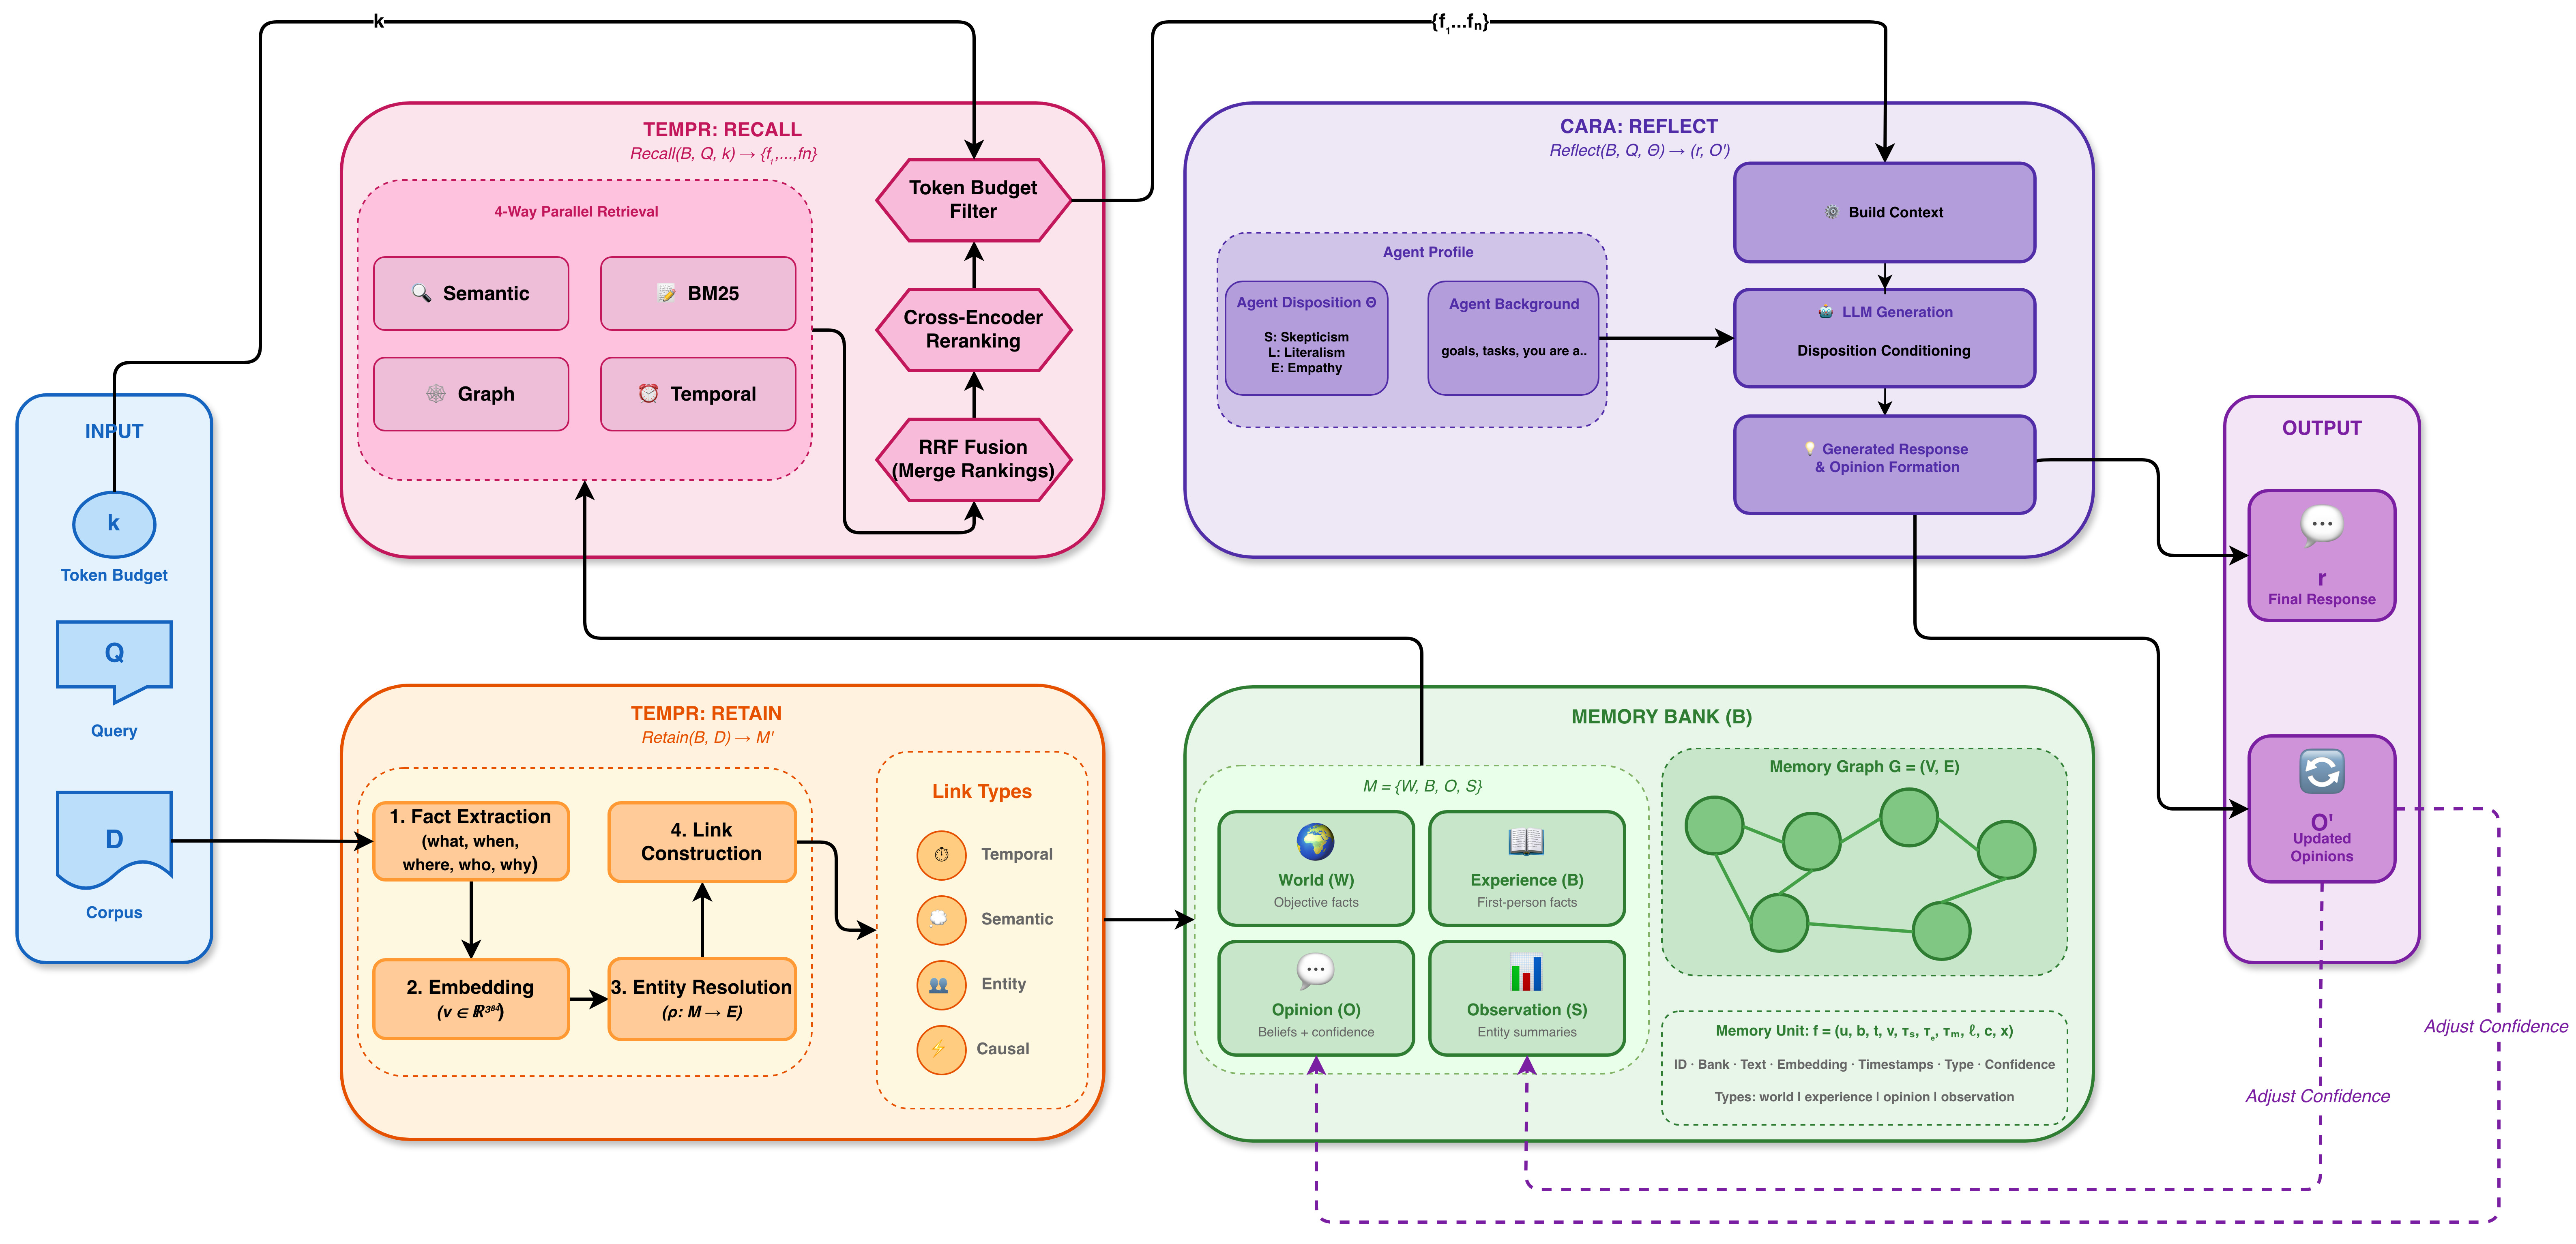
\includegraphics[width=\textwidth]{images/vectorize-hindsight.jpg}
    \caption{\textbf{End-to-end Hindsight architecture.} The system processes input data $D$ through TEMPR's retain pipeline (fact extraction, embedding generation, entity resolution, link construction) to build a structured memory bank $B$ containing four networks: world ($\mathcal{W}$), experience ($\mathcal{B}$), opinion ($\mathcal{O}$), and observation ($\mathcal{S}$). Given a query $Q$ and token budget $k$, TEMPR's recall pipeline performs four-way parallel retrieval (semantic, BM25, graph, temporal), applies Reciprocal Rank Fusion and cross-encoder reranking, and returns relevant facts. CARA's reflect operation takes these facts along with the behavioral profile $\Theta$ to generate preference-conditioned responses $r$ while forming and reinforcing opinions, updating the opinion network $\mathcal{O}'$.}
    \label{fig:hindsight-architecture}
\end{figure*}

\subsection{Component Architecture}

The two main components of \our implement these operations with distinct responsibilities:

\tempr realizes the retain and recall stages. It builds the four-network memory graph via LLM-powered narrative fact extraction, entity resolution, and link construction. TEMPR provides a retrieval interface optimized for agents, with token budgets and multi-hop discovery over temporal and entity-aware links. The retain pipeline processes input data by extracting narrative facts, generating embeddings, resolving entities, and constructing four types of graph links: temporal, semantic, entity, and causal.

\cara realizes the reflect stage. It integrates configurable disposition behavioral parameters into the reasoning process, operates over \our's networks to separate facts from beliefs, and maintains a dynamic opinion network via opinion formation and reinforcement. The behavioral profile consists of three disposition parameters (skepticism, literalism, empathy), each ranging from 1 to 5, and a bias-strength parameter between 0 and 1. CARA uses this profile to modulate the generation process, ensuring that responses align with the configured behavioral style.  Figure~\ref{fig:hindsight-architecture} provides a comprehensive view of the end-to-end architecture, showing the data flow from input through TEMPR's retain and recall pipelines, the four-network memory bank structure, and CARA's preference-conditioned reflect operation.



\subsection{Design Principles}

The architecture of \our is designed around several goals that recur throughout the paper. First, we aim for epistemic clarity, wherein
facts, observations, and opinions are kept structurally distinct so that developers and users can see what the agent knows versus what it believes. The four-network
organization
$\mathcal{M} = \{\mathcal{W}, \mathcal{B}, \mathcal{O}, \mathcal{S}\}$ provides explicit separation between objective evidence ($\mathcal{W}, \mathcal{B}$), subjective beliefs ($\mathcal{O}$), and synthesized summaries ($\mathcal{S}$). 
Second,
each memory unit $f$ carries temporal metadata $(\tau_s, \tau_e, \tau_m)$ where $\tau_s$ and $\tau_e$ define the occurrence interval and $\tau_m$ denotes the mention time, enabling precise historical queries and recency-aware ranking. This achieves
temporal awareness, wherein for a query with constraint $[\tau_{\text{start}}, \tau_{\text{end}}]$, the system retrieves facts where the occurrence interval overlaps with the query range. 
Third, this approach supports {\textit{Entity-aware reasoning}} leveraging graph links over shared entities, semantic similarity, temporal proximity, and causal relationships support multi-hop discovery of indirectly related information. The memory graph is the underlying data structure that connects all memory units: formally, $\mathcal{G} = (V, E)$ where $V$ is the set of all memory units (facts stored in the four networks) and $E$ is the set of weighted edges between them. Each edge $e \in E$ has a type $\ell \in \{\text{temporal}, \text{semantic}, \text{entity}, \text{causal}\}$ and weight $w_e \in [0,1]$, enabling traversal-based retrieval. Finally, \our aims for 
preference consistency, disposition behavioral parameters (skepticism, literalism, empathy) and a bias-strength parameter ensure that agents express stable perspectives over time while still allowing their beliefs to evolve as new evidence arrives, where the confidence score $c$ in each opinion $(t, c, \tau) \in \mathcal{O}$ is updated through a reinforcement mechanism when supporting or contradicting evidence is retained.

The following sections instantiate \our's architecture. Section~\ref{sec:tempr} describes TEMPR, which implements \our's retain and recall operations and builds the four-network memory graph. Section~\ref{sec:cara} then presents CARA, which implements the reflect operation and shows how preference-aware reasoning is layered on top of this memory substrate. Section~\ref{sec:hindsight-architecture} describes the unified integration of these components followed by experimental results.
